
\section{mclique2g.rb 極大クリークグラフの生成\label{sect:mclique2g}}

本コマンドは、一般グラフ(以下、「オリジナルグラフ」と呼ぶ)から列挙された各極大クリーク
\footnote{極大クリークの定義については\ref{sect:mclique}節を参照のこと。}
を節点とする新たなグラフ(「極大クリークグラフ」と呼ぶ)を生成する。
クリーク間に共通節点があれば、対応する接点間に枝を張る。

以下に例を示す。
図\ref{fig:clique2g_1}のグラフは4つの極大クリークを含んでいるが、
このグラフから図\ref{fig:clique2g_2}に示すグラフが生成される。
節点$0$は、図\ref{fig:clique}のクリーク\{$a,b,c,d$\}に、
節点$1$は\{$d,e,f$\}に、節点$2$は\{$e,f,g$\}に、対応している。
そして、節点$3$は\{$e,f,h$\}に対応している。

極大クリークグラフの節点$0$と$1$は、オリジナルグラフにおいて共通節点を1つ($d$)を持つので、節点$0$と$1$に枝が張られ、その重みが1となっている。
同様に、$1$と$2$は共通節点を2つ($e,f$)を持つので、節点$1$と$2$に枝が張られ、その重みが2となっている。
一方で、$0$と$2$は共通節点を持たないので、節点$0$と$2$には枝が張られない。

\begin{figure}[htbp]
\begin{center}
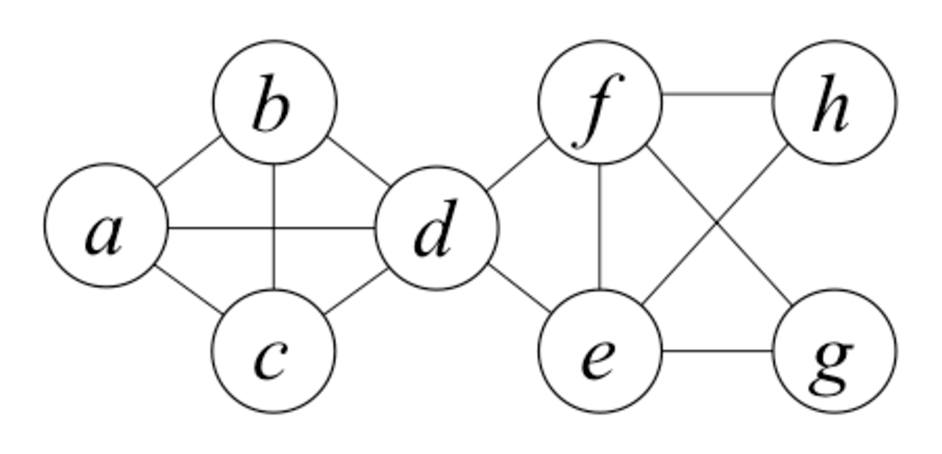
\includegraphics[scale=0.5]{./clique2g_1.eps}
\caption{4つの極大クリーク
\{$a,b,c,d$\}
\{$d,e,f$\}
\{$e,f,g$\}
\{$e,f,h$\}
が含まれる。
\label{fig:clique2g_1}}
\end{center}
\end{figure} 

\begin{figure}[htbp]
\begin{center}
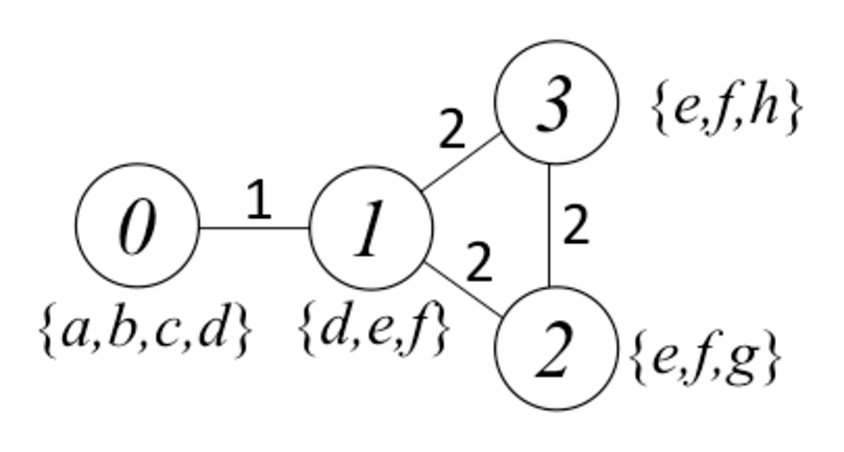
\includegraphics[scale=0.5]{./clique2g_2.eps}
\caption{新たに生成される極大クリークグラフ\label{fig:clique2g_2}}
\end{center}
\end{figure} 

さて、本コマンドの入力データであるオリジナルグラフは、表\ref{tbl:clique2g_1}に示されるような、
クリークIDと節点の2項目から構成されるCSV形式データである。
このデータは\ref{sect:mclique}節で示したmclique.rbコマンドで\verb|-node|を指定して出力されたデータに対応している。

そして、出力結果である極大クリークグラフは、節点データ(表\ref{tbl:clique2g_2})と枝データ(表\ref{tbl:clique2g_3})を別々に出力する。
節点データにおける\verb|weight|項目は、極大クリークを構成する節点数である。
また枝データにおける\verb|weight|項目は、極大クリークを構成する節点数である。

\begin{table}[htbp]
\begin{center}
\begin{tabular}{ccc}

\begin{minipage}{0.3\hsize}
\begin{center}
\caption{オリジナルグラフ\label{tbl:clique2g_1}}
{\small
\begin{tabular}{cc}
\hline
id&node \\
\hline
0&a \\
0&b \\
0&c \\
0&d \\
1&d \\
1&e \\
1&f \\
2&e \\
2&f \\
2&g \\
3&e \\
3&f \\
3&h \\
\hline
\end{tabular} 
}
\end{center}
\end{minipage}

\begin{minipage}{0.3\hsize}
\begin{center}
\caption{極大クリークグラフ(節点データ)\label{tbl:clique2g_2}}
{\small
\begin{tabular}{cccc}
\hline
node&weight \\
\hline
0&4 \\
1&3 \\
2&3 \\
3&3 \\
\hline
\end{tabular} 
}
\end{center}
\end{minipage}

\begin{minipage}{0.3\hsize}
\begin{center}
\caption{極大クリークグラフ(枝データ)\label{tbl:clique2g_3}}
{\small
\begin{tabular}{cccc}
\hline
node1&node2&weight \\
\hline
0&1&1 \\
1&2&2 \\
1&3&2 \\
2&3&2 \\
\hline
\end{tabular} 
}
\end{center}
\end{minipage}


\end{tabular} 
\end{center}
\end{table} 


\subsection{書式}
\begin{verbatim}
書式) mclique2g.rb i= [id=] [f=] eo= no= [T=] [--help]

  ファイル名指定
  i=  : クリークファイル名
	id= : クリークID項目名(デフォルト:"id")
  f=  : クリークを構成する節点項目名(デフォルト:"node")
  eo= : 出力枝ファイル名
  no= : 出力節点ファイル名

  その他
  T= : ワークディレクトリ(default:/tmp)
  --help : ヘルプの表示
\end{verbatim}

\subsection{利用例}
\subsubsection*{例1: 基本例}

前節で解説した例。


\begin{Verbatim}[baselinestretch=0.7,frame=single]
$ more clique.csv
id,node
0,a
0,b
0,c
0,d
1,d
1,e
1,f
2,e
2,f
2,g
3,e
3,f
3,h
$ mclique2g.rb i=clique.csv eo=edge.csv no=node.csv id=id f=node
#END# /usr/bin/mclique2g.rb i=clique.csv eo=edge.csv no=node.csv id=id f=node
$ more edge.csv
node1,node2,weight
0,1,1
1,2,2
1,3,2
2,3,2
$ more node.csv
node,weight
0,4
1,3
2,3
3,3
\end{Verbatim}


